\chapter{The HiSPARC Experiment}

\section{Design criteria}

% Explain why we want to detect cosmic rays; possibly identify sources (anisotropy)
Many unanswered questions remain in cosmic rays research. The main unresolved problem is the origin of cosmic rays. To find out which objects and by which processes are cosmic rays accelerated. This is difficult to determine for low energy charged cosmic rays, because their direction changes so drastically due to magnetic fields. However, direct observations of bremsstrahlung, synchrotron radiation, and neutral pion decay at the sources may reveal their origin, but that is out of the scope of this experiment. High-energy cosmic rays travel in straighter paths and may be used to backtrace to an origin.

% verifying GZ-effect
Composite cosmic rays may undergo spallation due to solar photons. In this process they break into smaller part which may produce simultaneous but geographically separated air showers. This is called the Gerasimova-Zatsepin (GZ) effect. This processes has not yet been conclusively detected. It is a rare process and requires simultaneous detections at very large (\SIrange{1e2}{1e4}{\kilo\meter}) distances, with good direction reconstruction of each shower.

% find features in the shower front, detect jets in air showers, e/mu ratio, temporal/lateral
The full shower development in the atmosphere is not fully understood. The shower front is the result of the interactions in the atmosphere. Understanding of the shower front provides better insight into what interactions happened in the shower development. For instance the existence of jets in the shower. Jets result in irregularities in the shower front at small scales. A fine grid of detectors is required to detect these irregularities. Also the temporal and lateral structure of the shower front require further investigation. By using high sampling frequencies the temporal structure may be unraveled.

% investigate relations to lightning strikes
Theories exists about a possible connection between lightning storms and cosmic rays. When the conditions are right for a lightning storm a cosmic ray air shower may be the initiator. Cosmic rays may help with ionisation of the atmosphere, providing a path for the lightning to strike. [CWI, LOFAR, RU]

% educate high-school students in research and physics.
Finally cosmic rays can be used to educate high school students. Currently subjects like quantum mechanics, relativity, electromagnetic fields, and particle physics are part of the `Nieuwe Natuurkunde' (NiNa) program for physics at high schools. `Natuur, Leven en Technologie' (NLT) is also a subject for students interested in physics. It consists of multiple domains from which students can choose, one of these is `Stellaire informatie en processen', which translates to Stellar information and processes. The data analysis also provides practical teaching material for informatics students. Cosmic rays provide an excellent teaching subject for these topics.

% Which cosmic rays do we want to detect, energy range; large area for very energetic cosmic rays, but also detectors close together for efficiently detecting low energy cosmic rays.
In order to efficiently detect high energy cosmic rays a large detection area is required (or a very patient researcher), because of the low flux. Individual detectors need to be spaced such that enough of the shower front is sampled to allow reconstruction of properties of the shower and primary cosmic ray. For low-energy cosmic rays the detectors need to be placed closer in order to sample the shower front. The flux of low energy cosmic rays is much higher, so much less total area is required to in a short time detect a lot of them.

For low energy showers the density drops off to rapidly and direction reconstruction will be hard when detectors are to close and the time resolution can not keep the angular resolution high. The energy range of interest is from \SI{e14}{\eV} and up. The upper limit will be determined by the final size and duration of the project.

\begin{figure}
    \centering
    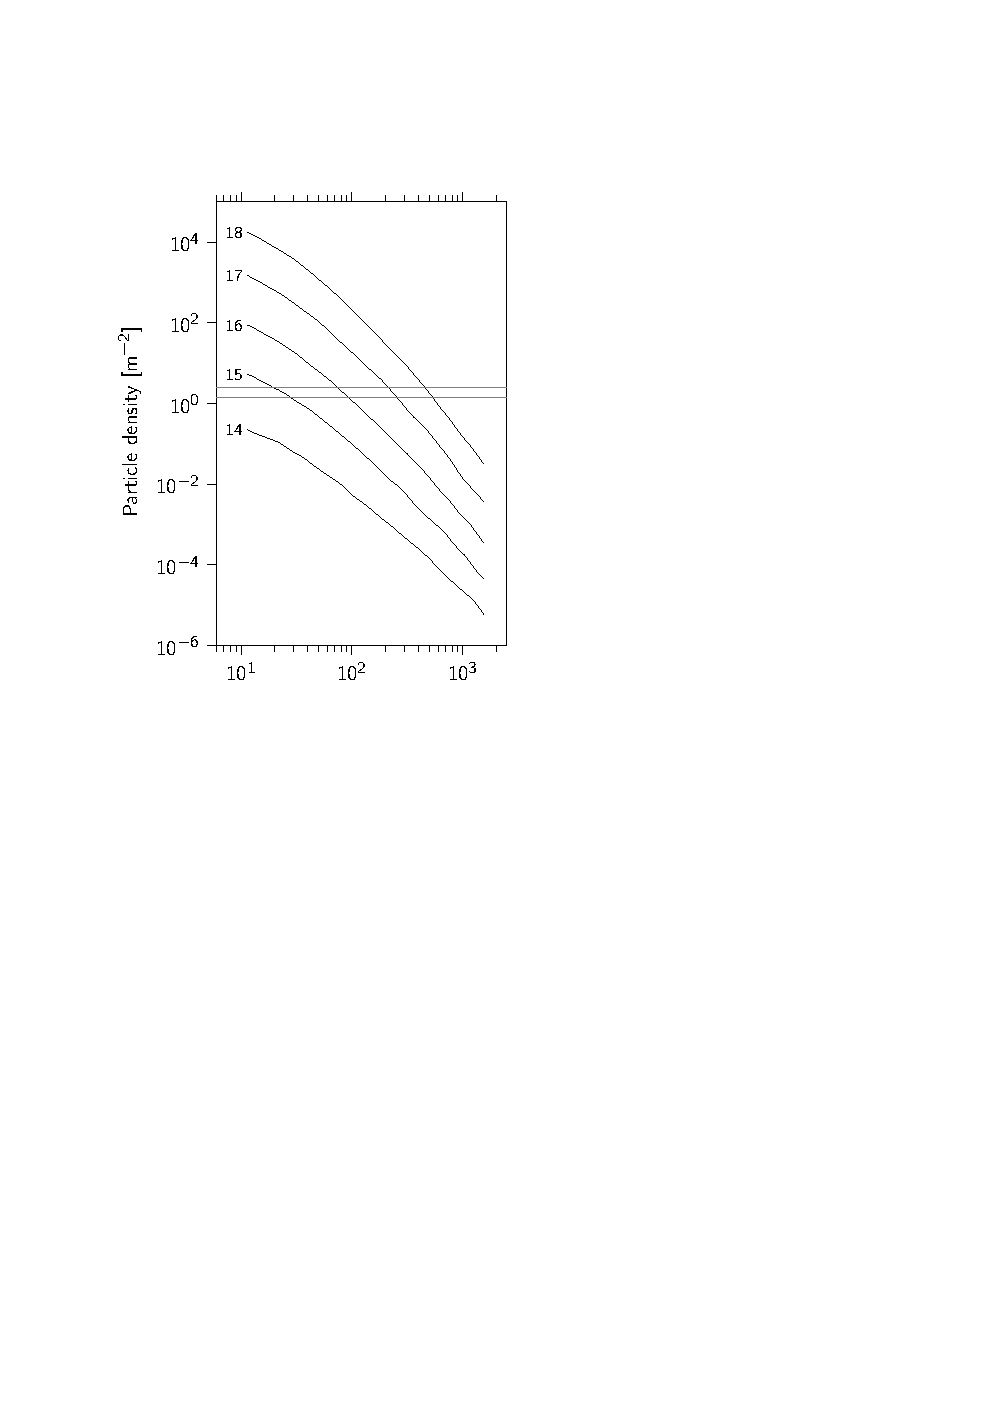
\includegraphics[width=0.6\textwidth]
                    {plots/experiment/ldf_energies}
    \caption{LDF for E = \SIrange{e14}{e20}{\eV} showers (e + mu). This gives the limits of detecting showers, depending on core distance and detector size. (do not show horizontal lines)}
    \label{fig:ldf_energies}
\end{figure}

% What do we want to determine for each air shower; time of arrival, direction of the shower axis, position of the core, and energy of the primary.
% Which properties of the shower need to be measured to determine this
By detecting the arrival time of particles from the same shower at various locations the shower front is sampled. This allows for the reconstruction of the shower. Using the arrival times the direction of the shower can be reconstructed. Using the density the core position and energy can be obtained. These reconstructions are not independent, knowledge about the core position improves direction reconstruction, and vice-versa shower axis direction makes the estimation of expected particle densities more accurate.

% What are the possibilities of identifying a source
The experiment will be based in the Netherlands, with possible extensions to other countries. From the Netherlands the Northern sky is observed. This provides a similar field of view to the TA experiment, which is at latitude \SI{39.3}{\degree}, while \nikhef is at \SI{52.3}{\degree}. The visible-sky map, assuming a zenith acceptance of \SI{60}{\degree}, in equatorial coordinates is shown in \cref{fig:visible_sky_map}. The anisotropy measurement of cosmic rays at very high energies is difficult to achieve. The Auger and TA experiments have only a handful of detections above \SI{e20}{\eV}. These experiments have exposures of \SI{7250}{\kilo\meter\squared\year\steradian} (TA) and \SI{48029}{\kilo\meter\squared\year\steradian}, which is a meaure of their area, angular acceptance, and run time. Measurement of the isotropy at lower energies is important for verification of the expectation.

\begin{figure}
    \centering
    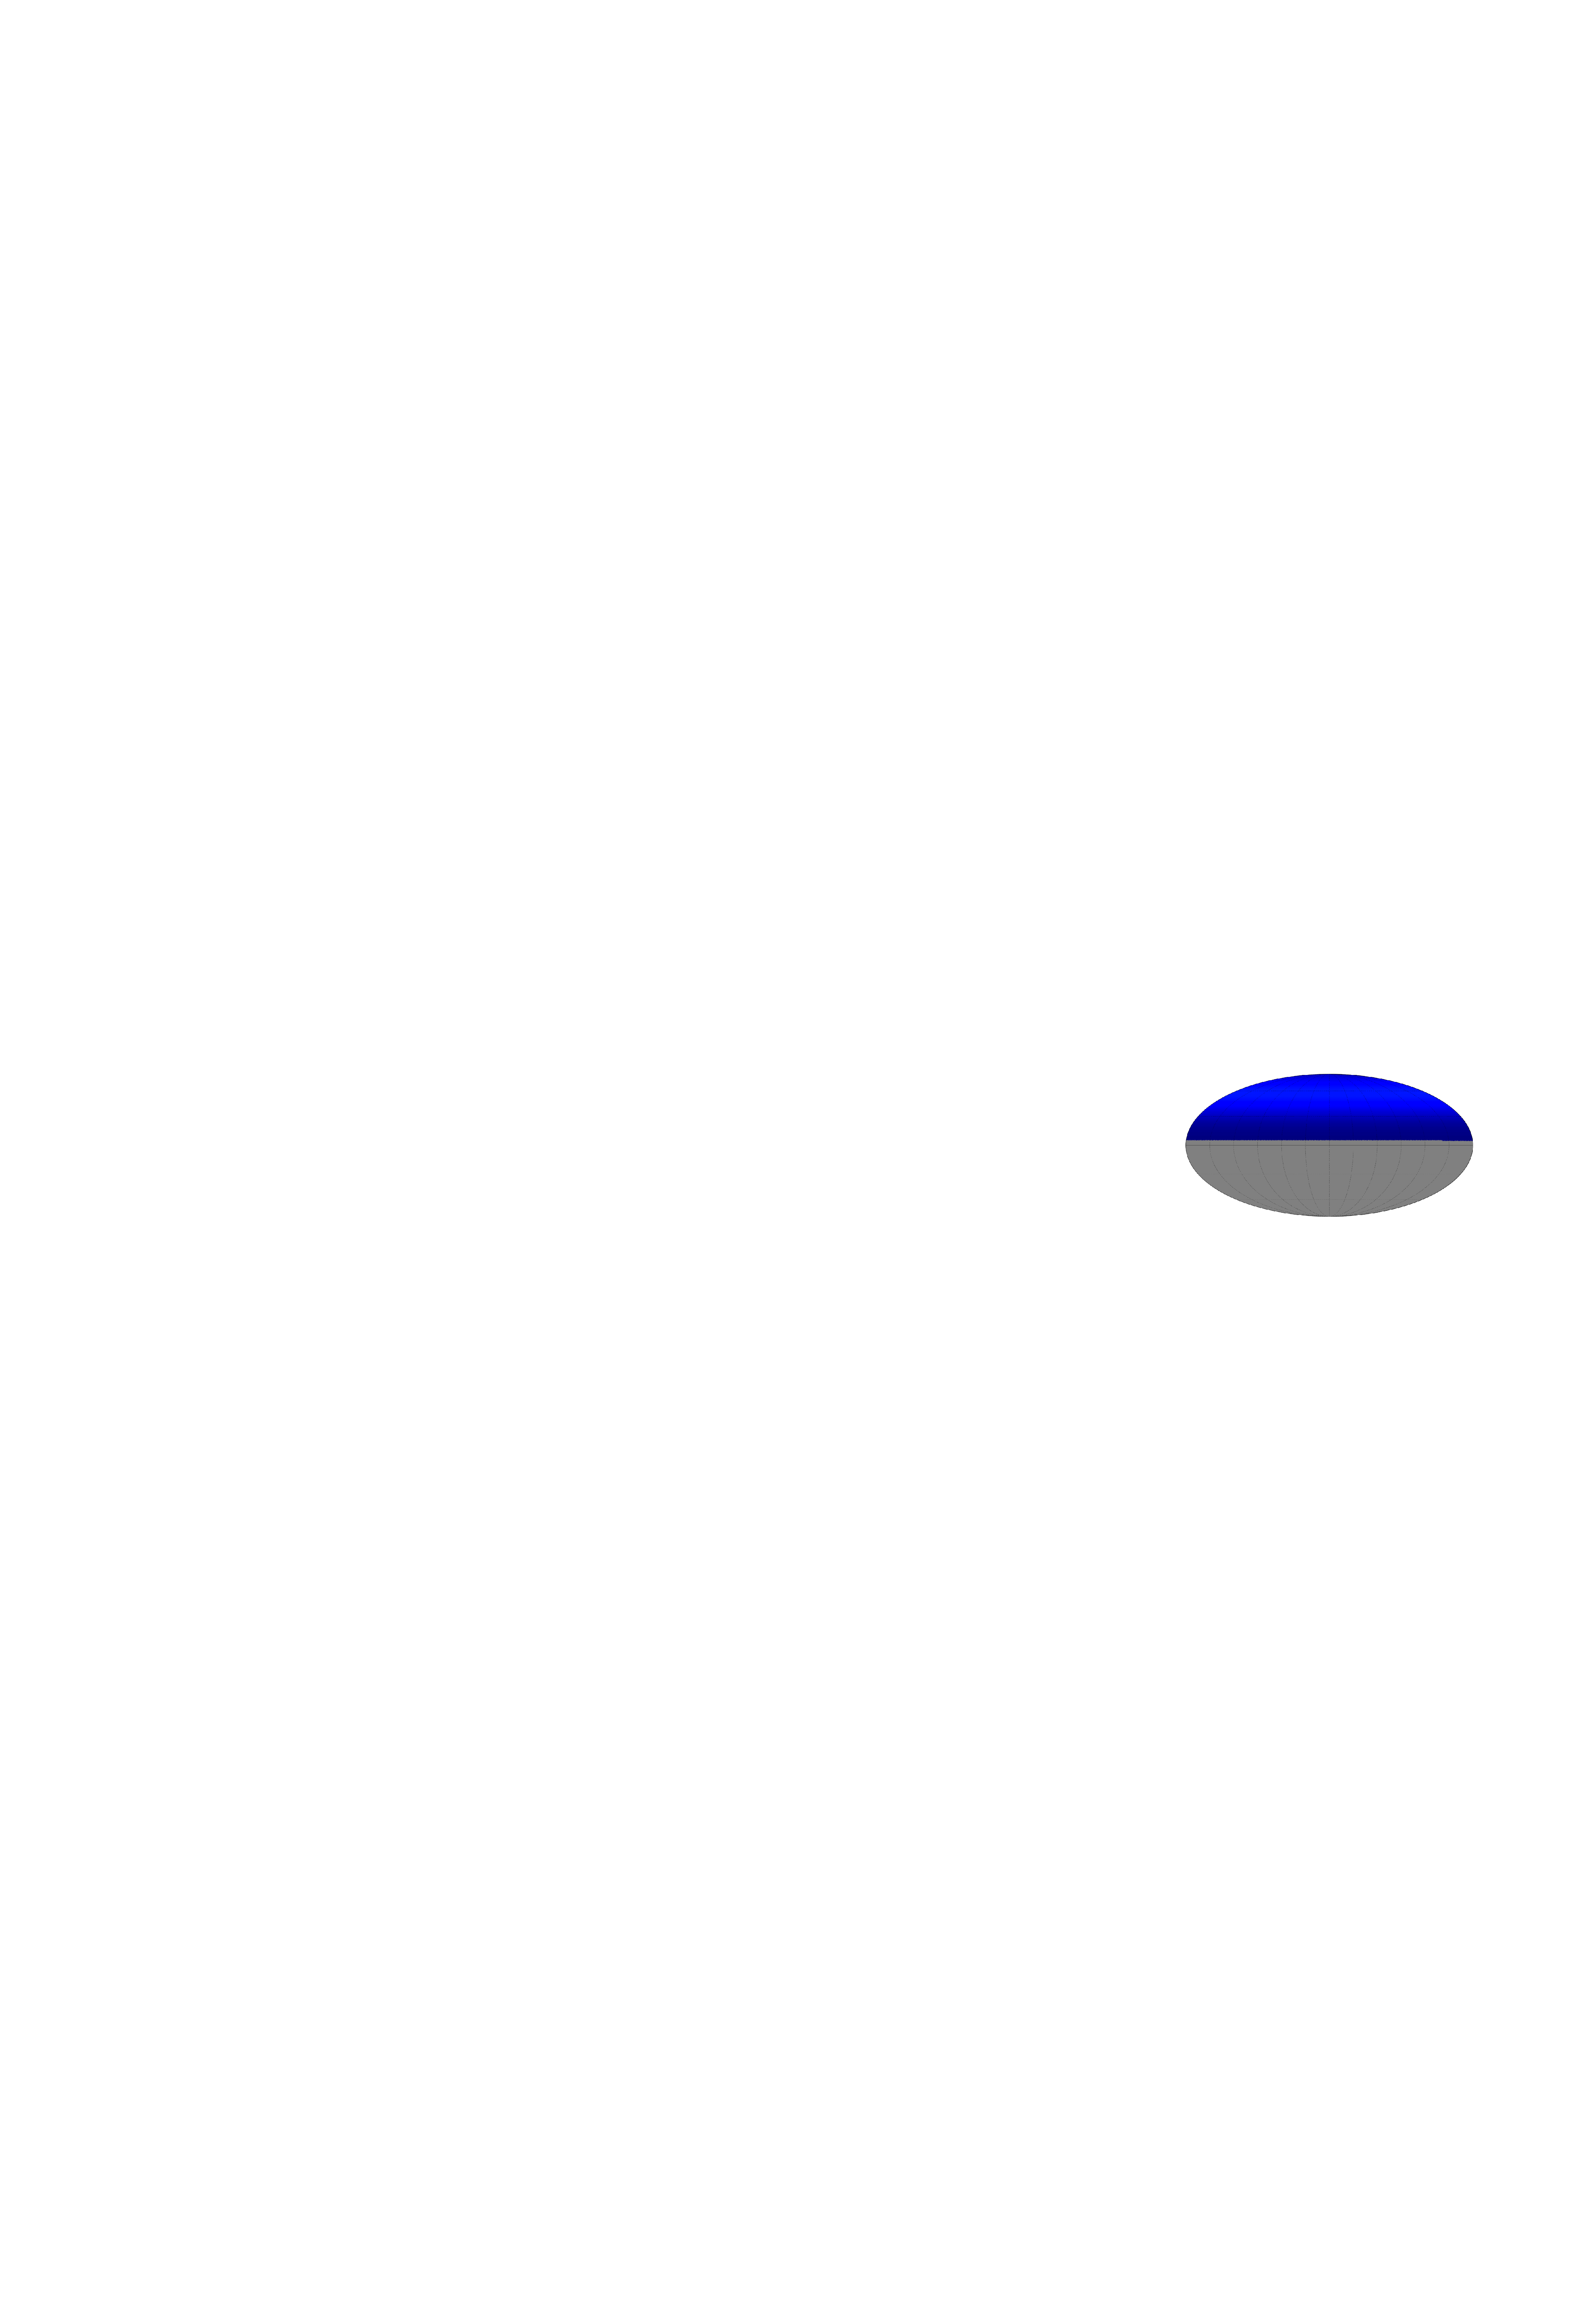
\includegraphics[width=0.6\textwidth]
                    {plots/experiment/visible_sky_map}
    \caption{Equatorial sky map (mollweide) highlighting part of universe which is above the horizon in the Netherlands. Similar field of view to TA/KASCADE.}
    \label{fig:visible_sky_map}
\end{figure}


\section{Design for detection}

% Detector the particles in the shower front, not the fluorescence/Cherenkov. For several reasons; particle detectors are much cheaper, provides higher uptime. Also detect extensive air showers during day time, moon nights, and with other sources of light pollution.
In \cref{sec:other_observables} methods other than particles detectors for the observation of air showers were mentioned. These will not be considered, as these methods are much more expensive and have lower duty cycles. For experiments such as TA and Auger they do provide excellent independent calibration of the surface particle detectors and extra information about the shower. This experiment will use particle detectors for the detection of cosmic rays.

% What properties/observables of the air shower particles need to be measured.
%  - Arrival time of the particles (leptons) and their number.
%  - Accurate arrival time is needed for direction (using shower front shape).
%  - Accurate particle count is needed for energy/core (using lateral density).
The arrival time of particles and number of particles in a detector can be used to reconstruct the shower. The accuracy with which this can to be measured depend on the properties of the shower and detectors. For increasing distance between detectors a lower arrival time accuracy is required to achieve the same direction reconstruction accuracy. With increasing core distance the particle density decreases, while the rise time of the shower front increases. This makes it more likely that the few particles that are detected are further delayed from the causal front. This increases the uncertainty in direction reconstruction.

Important to consider is the likelihood of actually detecting a shower. For a given charged particle density $\rho$ and a detector with area $A$ the probability of detecting exactly $k$ particles is given by the Poisson distribution. Here $\lambda$ is the expected number of particles, i.e. $\lambda = \rho A$ and $P_k$ the probability.
%
\begin{equation}
    P_k(\lambda) = \frac{\lambda^k \mathrm{e}^{-\lambda}}{k!} \ .
\end{equation}
%
This assumes the detectors are \SI{100}{\percent} efficient at detecting charged particles. The important probability is the probability of not detecting any particle (i.e. $k = 0$) given a particle density, given by
%
\begin{equation}
    P_0(\lambda) = \mathrm{e}^{-\lambda} \ .
\end{equation}
%
Which gives the probability of detecting at least one particle via
%
\begin{equation}
    P_p(\lambda) = 1-P_0(\lambda) \ .
\end{equation}

% Each particle detector will have a background from low energy showers, such showers are very abundant, but only few particles (mainly muons) reach ground level.
Not all detected particles will be desired. A big component of the background comes from low energy showers (\SI{<e14}{\eV}) which produce only a couple muons at sea level, and even fewer electrons. Such low energy cosmic rays are very abundant. Instead of resulting in an instantaneous high density of particles these showers produce a random background of particles. These showers produce to few particles to effectively sample the shower front. In \cref{fig:particle_density} the total particle flux at various atmospheric depths is shown. At sea level the muon flux dominates. The high muon flux relative to electrons is dominated by low energy showers, for higher energy showers the electron-muon ratio favors the electrons.

\begin{figure}
    \centering
    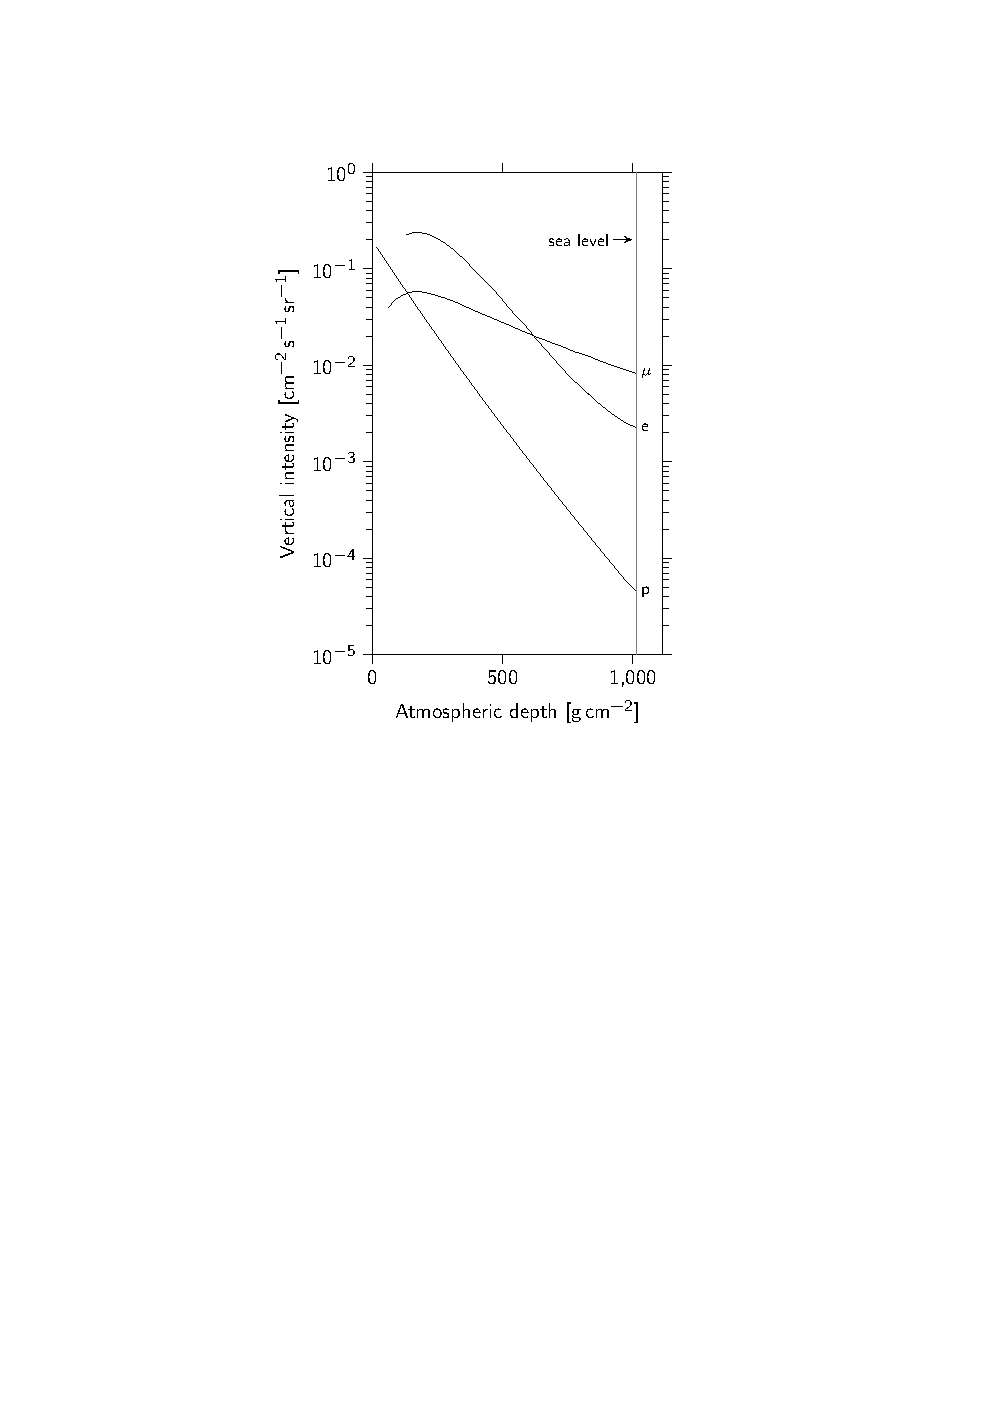
\includegraphics[width=0.6\textwidth]
                    {plots/experiment/particle_density}
    \caption{Particle flux composition as function of atmospheric depth, to show the flux of particles at ground level, todo: filter for only particles with 'enough' energy (like Grupen fig7.10)}
    \label{fig:particle_density}
\end{figure}

% How to filter the background away by using a coincidence trigger. Two (or more) simultaneous, unrelated, detections in separated detectors is unlikely.
By using the fact that the particles from energetic showers are more correlated in time those showers can be distinguished from the background by looking for time-correlated particles. This might be possible with a single detector which looks for short bursts of many particles. However, this does not provide data for reconstruction, since the arrival time and density is only known at one position. Multiple combined detectors using a time-correlated trigger is more sensitive to lower particle densities, since one particle needs to be detected per detector. Moreover, it provides data for reconstruction. Using two detectors to distinguish the particles from the background by requiring at least one particle in each detector makes the probability detection $P_2(\lambda) = P_p^2(\lambda)$, assuming the particle density is equal at both detectors. The size of and distance between the detectors will determine the lower energy limit.

% How to figure out where should the detectors be placed (relative to each other)
%  - For low energy (\SIrange{e14}{e15}{\eV}) showers the detectors need to be closely spaced (\SI{10}{\meter}) otherwise the density in the detectors becomes to low to effectively detect them.
%  - For high energy (\SIrange{e18}{e20}{\eV}) showers the detectors need to be placed further apart (\SI{>500}{\meter}) otherwise the area covered by the detectors is to small and only few high energy showers will be detected.
The efficiency with which two detectors can detector a shower can be estimated. Assume that the shower core is precisely between the two detectors. Here the detection efficiency is highest. If the shower was closer to either detector the probability of detection for one detector would go up, but it falls faster for the other detector, reducing the overall probability. Using an estimate of the particle density for (vertical) showers as described in \cref{eq:nkg} the probability of detection can be estimated for showers of different energies depending on the size of the detectors and the distance between the detectors.

The relation between the median shower size (number of electrons at sea level) and primary energy (see \cref{fig:shower_size_distribution}) can be approximated by the following relation
%
\begin{equation}
    N_{\Pe} = 10^{\log\left(\frac{E}{\si{\eV}}\right) - 10.2} \ ,
\end{equation}
%
which is valid for (semi-)vertical showers. As the zenith angle of showers increases above \SI{15}{\degree} the shower size noticeably decreases. Also the energy at which the transition from mostly muons to mostly electrons reach ground is at higher values for larger zenith angles. A better fit may be achieved by adding an extra parameter
%
\begin{equation}
    N = 10^{\log\left(\frac{E}{\si{\eV}}\right)^y - x} \ .
\end{equation}
%
This can be fitted more accurately to the electron, muon and total lepton sizes (per zenith angle). For electrons the values $y = 13.3$ and $x = 1.07$ best describe simulated air showers (protons from the Zenith).

$P_2$ is a function of $P_0$, which can be written as a function of the shower energy, core distance, and detector size as follows
%
\begin{equation}
    P_0(E, r, A) = \mathrm{e}^{-A\rho(N_{\Pe}(E), r)} \\ .
\end{equation}
%
With this the expected detector efficiency for a detector setup can be estimated for various shower energies. Inclined showers can also be investigated, in case of a flat detector the effective detection area is smaller by $\cos \theta$. The particle density is harder to estimate because different parts of the shower have different path lengths through the atmosphere. Also the effective distance between the detectors may change, depending on the azimuthal angle of the shower.

% Why are for reconstruction multiple detection points needed.
To be able to fully reconstruct the direction of an air shower at least three detection points are required. Having two detection points with arrival times provides a constraint on the shower axis, but a plane of possibilities remain \cite{schultheiss2016pair}, a third detection point (not on the same line) constrains the shower axis. This can either be achieved by a single station with three or more detectors (short distances), or by combining detections from multiple stations (larger distances). Using a 3-detector station the probability of detecting at least one particle in each is given by $P_p^3(\lambda)$. If the station had even more detectors ($n$) but still required at least 3 in coincidence the probability of detection becomes
%
\begin{equation}
    P_{\mathrm{min}=3}(\lambda) = \sum_{k=3}^{n} \binom{n}{k} P_p^k P_0^{n-k} \ .
\end{equation}

% Depending on size of coincidence window how much background remains. Reconstruction should identify bad/accidental events.
Consider the 2-detector setup again in which both need to detect a particle within a short time window to make certain both are from the same shower. The rate of muons at ground level is approximately $f_{\Pmump} = \SI{~200}{\Pmump\per\meter\squared\per\second}$. Most should have entirely uncorrelated arrival times. Since the distribution is random some might arrive simultaneously. The expected rate of random coincidences can be calculated by
%
\begin{equation}
    \label{eq:background_rate}
    R_{\mathrm{background}} = 2 \tau A^2 f^2 \ ,
\end{equation}
%
where $\tau$ is the time window, $A$ the detector area, and $f$ the background flux. Note that this relation is only applicable if the time window $\tau$ is smaller than $f^{-1}$ and $R_{\mathrm{background}} \ll Af$.

The time window should be at least the distance between the two detectors divided by the light speed. That should be the most extreme case for a shower to arrive horizontally in line with the detectors. Longer time differences are possible due to different transport time in the detector and the rise time and curvature of the shower front.

% The detectors need to be reliable to prevent continuous maintenance tasks, and to last the length of the experiment, MoU expects ~5 years.
Ideally the detectors operate without maintenance. The components might have finite lifetimes or require recalibration after some time. If many detectors require frequent service and maintenance this will cost time that could otherwise be spent on data analysis. Basically the costs of the experiment go up. Using tried-and-tests components that have been shown to be reliable for long periods are preferred.

% Cost effective detectors so high-schools can participate in the project
Making detectors larger makes them more likely to detect particles. The downside is that the detector becomes less easy to handle, more expensive, efficiency uniformity may worsen, and saturation might occur sooner. A good balance needs to be determined.

% The detector needs to be safe to handle by students
% Detectors need to be durable so they can survive the typical Dutch weather
The experiment is meant to be accessible for high schools, the detectors need to be fairly easy to handle. If the detectors would be placed inside schools it may be difficult to find a safe location and the roof material might affect the detections. In order to have enough space to place the detectors the most obvious location would be on the roof. If the detectors are outside proper protection from weather effects need to be considered.


\section{Detector}

% Using scintillators with PMTs provide good particle detection efficiency, \SI{100}{\percent} of energetic leptons are detected, also some gammas are seen.
The detector consists of two main components which perform the detection. The scintillator, which emits light when charged particles pass through it, and the Photomultiplier tube (\pmt) which converts the scintillation photons into an electric signal.

% Scintillator size and material
Scintillators have been selected as detection material. This is a relatively cheap material with high reliability and excellent efficiency. The scintillator is a sheet of \SI[product-units=power]{100 x 50 x 2}{\centi\meter} made from BC-408 \cite{bc408}. The BC-408 material has good timing properties and light output for charged particles.

% PMT size and type
The chosen photomultiplier tube \cite{et:pmt} is a compact \SI{29}{\milli\meter} (\SI{25}{\milli\meter} effectively) diameter and \SI{~11}{\centi\meter} long (depends on the power supply) \pmt. The quantum efficiency of the biakali photocathode is \SI{25}{\percent} for the wavelength of maximum emission of the scintillator, which is \SI{425}{\nano\meter}. The \pmts contain a number of high gain caesiated antimony (SbCs) dynodes. The \pmts are very efficient at amplifying faint light pulses to measurable electric signals. Several brands and types of \pmts have been used. At first \pmts (including power supply) were sourced from Electron Tubes, ET Enterprises and Sens-Tech, later new \pmts were constructed using Hamamatsu tubes with a \nikhef power supply. The \nikhef power supply is also compatible with the previously used tubes, and can serve to replace a failed power supply.

Besides these the detector construction consists of several other components. An isosceles triangle light guide [measurements, base \SI{50}{\centi\meter}, legs ??, thickness ??] made from polymethylmethacrylate (PMMA). The light guide is glued to the scintillator using Optical Cement (\cite{bc600}). A little adapter piece (same material as light guide) is attached to the square end of the triangle with Optical Cement and the round window of the \pmt with optical tape [type?]. This construction is wrapped in thin, \SI{30}{\micro\meter}, aluminium foil with patches of thicker, ??, aluminium foil at the corners of the scintillator, to prevent the sharp edges from piercing the thin foil. This is then wrapped in thick, ??, light-tight black pond foil to keep light out and protect the aluminium foil from outside influences.

% Material is mostly 'off the shelf'. Construction/assembly can be performed by students.
All components are readily available, off the shelf, from suppliers and not specifically designed for \hisparc.

\begin{figure}
    \centering
    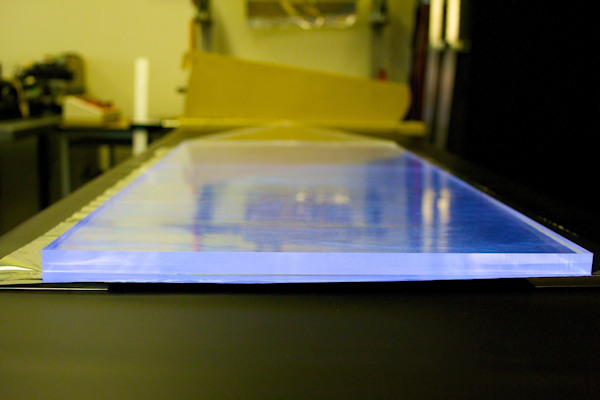
\includegraphics[width=0.6\textwidth]
                    {plots/experiment/ADL_115651.jpg}
    \caption{Show a schematic/photo of detector, indicating the various components.}
    \label{fig:schematic_detector}
\end{figure}

% Detector is protected by skibox from weather and is secured in place by weights.
The final detector dimensions (approximately \SI[product-units=power]{200 x 50 x 3}{\centi\meter} fit well in the chosen detector casing, namely, roof boxes (in Dutch generally referred to as `ski box'). These can be securely fastened and are designed to withstand all kinds of weather. Access to the detector for maintenance is also easy. Also with maintenance in mind, the optical tape with which the \pmt is attached allows it to be easily replaced.

[insert photo of detector in skibox]


\subsection{The scintillator}

% How Scintillator works
Charge particles loose energy in the scintillator in interactions with the base of the scintillator, polyvinyltoluene. Ionisation is the main source of energy loss for energetic charged particles (electrons, muons). The base will emit photons which are rapidly absorbed by the fluor of the scintillator, anthracene. The fluor then emits light at a lower wavelength, to which the scintillator is more transparent. Some of this light will reach the \pmt.

% Most shower muons/electrons are minimum ionising particles (mips) and have similar energy loss in the detectors, given by Bethe-Bloch (spread on energy loss given by Landau).
The average energy deposited by the particle going through the detector is described by the Bethe-Bloch formula. This gives the amount of energy lost by the particles per \si{\gram\centi\meter\squared} of the material it passes through. However, the interactions in which the particles loose energy is a statistical process, the energy loss is not a fixed number but a distribution, the Landau distribution. The ionisation energy loss (predicted by Bethe-Bloch) for both electrons and muons reaches a minimum value at some point. Muons and electrons at this energy (\SI{325e6}{\eV} and \SI{e6}{\eV} respectively) are referred to as \textit{minimum ionising particles} (\mip). In [figref] the energy loss for electrons and muons is shown as a function of their energy. Shown are the total losses (grey), losses due to ionisation (black), and other loss processes. The ionisation losses are the only ones of real interest, since those result in the detectable scintillation light.

[insert fig of energy losses, Bethe-Bloch, highlight ionisation, use eV horizontal scale (two scales?) or beta gamma..]

The scintillator is \SI{2}{\centi\meter} thick, however, many particles have a longer path through it because they travel at an angle. This increases the expected mean energy loss. The path can also be shorter if the particle passes through one of the sides of the scintillator, but due to the large area of the detector relative to its thickness the chance of that happening is low.

% Signal transport efficiency not uniform for the detector due to geometry.
The light emitted along the path of the particle is transmitted in random directions. Depending on the angle at which the emitted photons hit the outer edges of the scintillator there is a chance that they will be reflected back or leave the scintillator. The entire detector is wrapped in aluminium foil to attempt to reflect those photons back into the scintillator. To detect the photons they need to hit the photocathode of the \pmt. To get to the \pmt they need to pass from the scintillator through a layer of optical glue, the light guide, another layer of optical glue, a small piece of light guide, and a layer of optical tape to reach the \pmt. During this most photons will be reflected a number of times. For \SI{1}{\mip} approximately 30000 photons [check.] are emitted, the fraction that reach the \pmt depend on the location in the scintillator where the particles are emitted. A 2D Monte Carlo simulation of the detector [cite Jos Steijger] predicts the transmission efficiency from locations in the scintillator to the \pmt. The resulting transmission efficiency distribution is shown in [fig of transmission efficiency]. Also the travel time of the photons to the \pmt varies depending on the location of emission and the emission direction. In \cref{fig:transport_time} the distribution of transport times is shown, the time is the arrival time of the 15th photon producing a photoelectron at the \pmt. This is taken instead of the first because the signal threshold used for detection is greater than the signal of one photoelectron. The effects of these distributions on the reconstruction accuracy are discussed later.

\begin{figure}
    \centering
    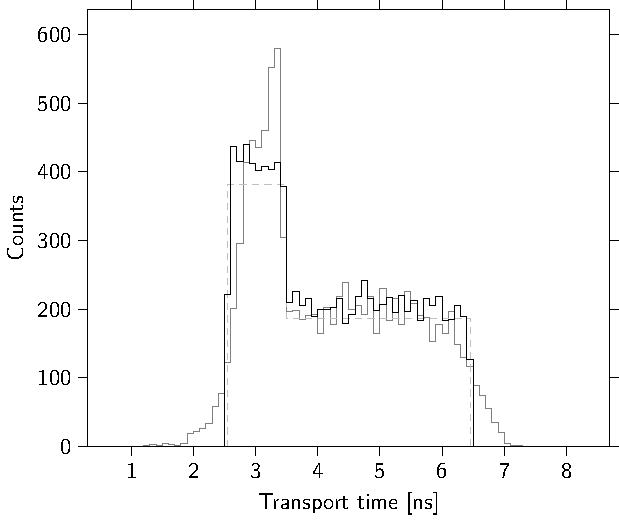
\includegraphics[width=0.6\textwidth]
                    {plots/experiment/transport_time}
    \caption{Transport time distribution for the detector. The scintillation light has to reach the PMT from the point of impact, the travel time depends on the impact location, this is the distribution for the entire detector.}
    \label{fig:transport_time}
\end{figure}


\subsubsection{Gammas in the scintillator}

Energetic photons can also deposit energy in the scintillator due to Compton scattering and pair creation. However, the cross sections for these interactions is very low. A \SI{e6}{\eV} photon  has a mean free path greater than \SI{10}{\centi\meter}, which increases further for higher energy photons, see fig [By Jos/Tom]. Despite the low detection chance, the large number of photons in an air shower makes them statistically relevant.

For photons the interactions by which it produces detectable signals are .., and pair production. In case electrons are produced, those will proceed in the usual way.


\subsection{\pmt}

% How PMT works
The photomultiplier tube has a front window with a photocathode. When this is hit by a photon an electron can be knocked free, due to the photoelectric effect. The electron is then pulled along electric field lines which direct it to a dynode. The electron will cause multiple electrons to be emitted from the dynode, these electrons are then pulled to the next dynode, which has a higher positive potential. Each electron impacting the second dynode will cause the release of more electrons, which are accelerated towards the next dynode, and so on. At the end the electrons fall on the anode which is connected to the readout. The \pmts which are used have 11? (ET/SensTech) and 12? (Hamamatsu) dynodes, this number affects the gain of the \pmt. If each electron causes \num{3} electrons to be released from a dynode then every electron falling on the first dynode will result in $3^{n_{\mathrm{dynodes}}} = \mathcal{O}(10^6)$ electrons at the anode. The number of electrons emitted by a dynode for each electron that falls on it is not a fixed number. This results in a variation in the output signal for each single photoelectron. This can easily vary a factor of 2, if for instance the first dynode emits either 2 or 4 electrons instead of 3. It is more likely to happen at a later dynode because more interaction occur at those. Typical variations are of the order of \SI{10}{\percent}. By changing the voltage on the dynodes the gain of the \pmt can be tuned, with a higher voltage resulting in a higher gain. The relation between gain and voltage is not linear [perhaps a fig, or at least a ref]. 

[schematic figure of \pmt]

% Signal strength is used for particle density, need to be able to distinguish between different number.
Both the scintillator and \pmt can handle multiple particles simultaneously and will produce correspondingly higher signal output. The integrated signal strength should be the sum of two individual particles. Given the signal distribution for single particles given by the Landau distribution combined with the transport efficiency one particle will in some (how often?) produce a signal equal or larger than the most probable signal strength of two particles. In \cref{fig:ph_histogram_contrib} an example of the expected pulse height histogram is shown including the contributions from gammas, and multiple leptons. The widths of the contributions are due to the particle inclination, Landau distribution, transmission efficiency, and \pmt variation. The first peak gives the most probable value (MPV) for the pulse height of a single lepton. An approximation of the number of particles can be made by comparing a measured value to the MPV. The position of the MPV is dependent on the efficiency of the detector, by changing the voltage on the \pmt the position of the MPV can be tuned. Ideally the MPV is approximately \SI{150}{\mV}. If it is lower it is difficult to distinguish the lepton contribution from the gamma spectrum and the MPV will be hard to determine. If the MPV is at a much higher value the \pmt ages more quickly and the dynamic range [in number of particles..] will be reduced.

\begin{figure}
    \centering
    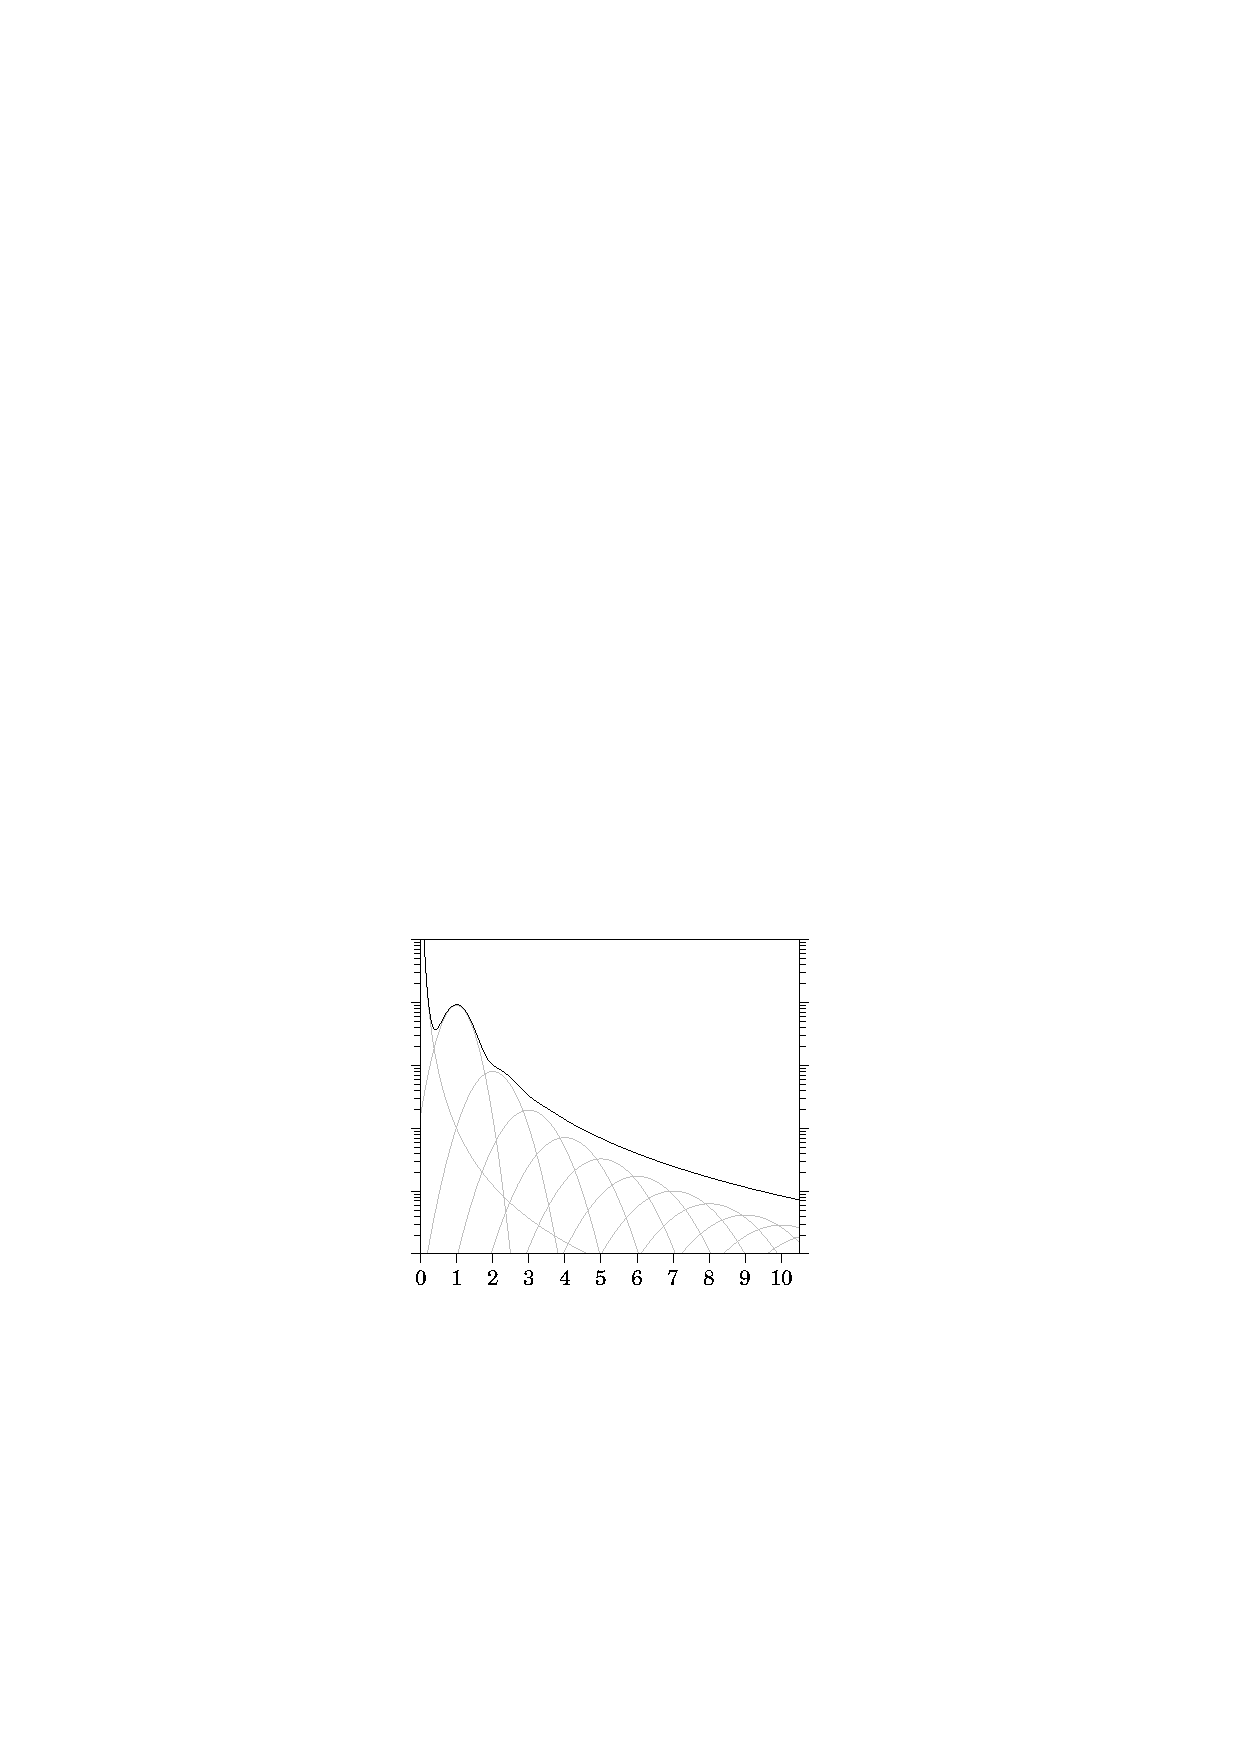
\includegraphics[width=0.6\textwidth]
                    {plots/experiment/ph_histogram_contrib}
    \caption{Overlap between pulse integral contributions from multiple mips in one event, the with of each contribution is due to Landau distribution and transport efficiency.}
    \label{fig:ph_histogram_contrib}
\end{figure}

% Fast ADC readout of the PMT provides accurate timing.
Each \pmt is readout with \adcs at a sample rate of \SI{2.5}{\ns}. An example of a readout is shown in \cref{fig:trace}. With this high sample rate the signal shape of individual particles is unraveled. Subsequent signals from particles later in the shower front can be distinguished, and the shower rise time can be examined. With \SI{2.5}{\ns} the timing resolution is close to timing the uncertainty caused by the shower front rise time and the detector transport time. An even higher sample rate would not achieve much better timing resolution.

\begin{figure}
    \centering
    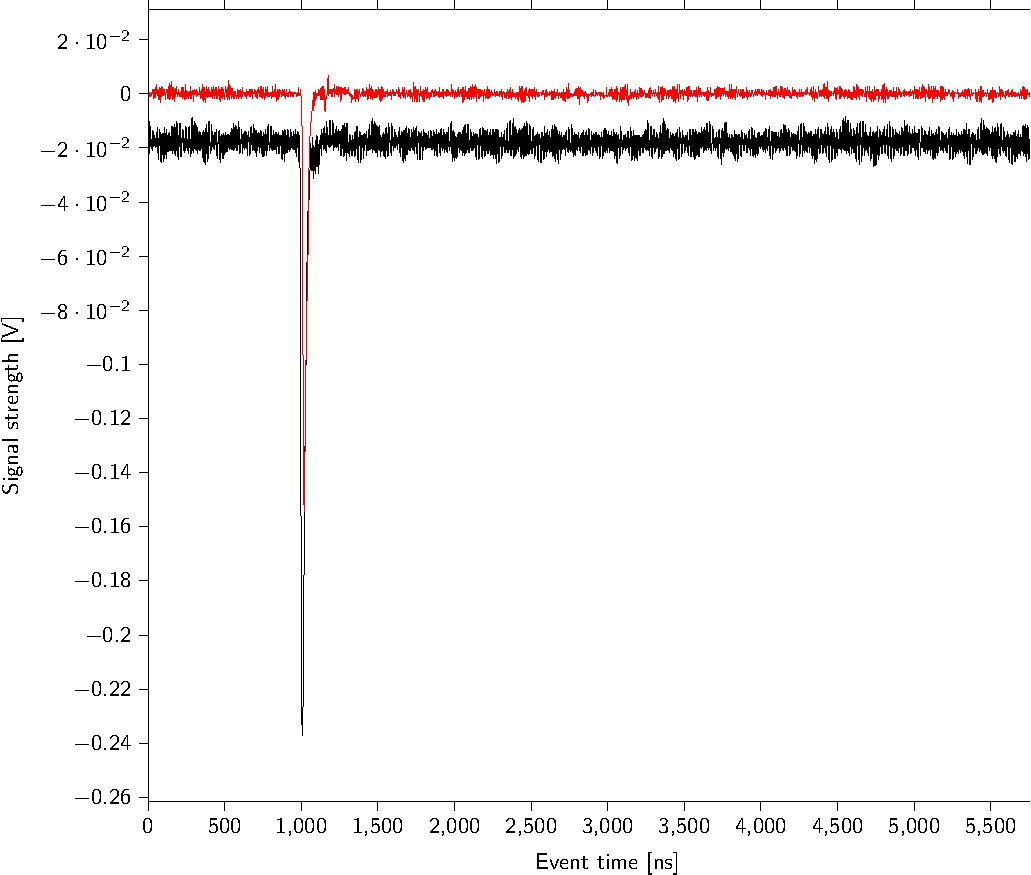
\includegraphics[width=0.6\textwidth]
                    {plots/experiment/trace}
    \caption{An example trace readout of the \pmt. The signal has the height of one \mip, so most likely one lepton was detected.}
    \label{fig:trace}
\end{figure}


\section{Station}

% Impractical to connect detectors over long distances for online/realtime triggering.
By making each detection station consist of at least two detectors the station can perform triggering as a standalone unit. Each station performs its own triggering, therefore stations do not need to be interconnected. For detection stations separated by large distances this approach is more practical, since wireless and wired communication are either to unreliable or to slow. For experiments like Auger where the space between detectors is mostly empty wirelessly connecting detectors is an option. The \hisparc station consists of either 2 or 4 detectors connected to \hisparc electronics. The \hisparc electronics incorporates \pmt readout and control, triggering logic, a \gps module, and a data connection to a PC. Two versions of the electronics are currently being used, versions II and III. Version III differs from II in having USB 2 (\SI{480}{\mega\bit\per\second}) instead of USB 1.1 (\SI{12}{\mega\bit\per\second}) connectors, slightly different \adcs, and an upgradable firmware over USB. The PC connected to the electronics contains software to send and receive messages to and from the \hisparc electronics. The message formats and their meaning are described in [hipsarc messages Verkooijen], further description of the software running on the stations is described in [later chapter].

\subsection{Signal readout}

The \hisparc electronics has two \adcs per channel, each reads the \pmt signal at \SI{200}{\mega\hertz}. By interlacing the two \adcs a sampling frequency of \SI{400}{\mega\hertz} is achieved. These are 12-bits \adcs, allowing values between \SIrange{0}{4095}{\adc} and provide approximately \SI{2}{\volt} dynamic range. The two \adcs are calibrated to provide the same baseline and gain. The baselines are set to \SI{200}{\adc} (II) and \SI{30}{\adc} (III) for the two \hisparc electronics. The two versions use a different type of \adc, with a slightly different dynamic range. The \si{\mV} to \si{\adc} conversion differs slightly, being \SI{0.57}{\adc\per\mV} (II) and \SI{0.584}{\adc\per\mV} (III). In addition to the \adcs each channel has two comparators which record the time over threshold for a given threshold. The thresholds of the comparators can be configured but are by default set to \SI{-5}{\volt} and \SI{-10}{\volt}. In case of signals which saturate the \adcs the comparators provide additional information about the actual signal size.

The \pmt signals are continually read out, the resulting \adc values are compared to two thresholds; a low and high threshold. These thresholds can be set for each channel individually. Usually they are set equally for all channels in a station, and the default setting is \SI{-30}{\milli\volt} (low) and \SI{-70}{\milli\volt} (high). The triggering logic keeps track of which channels are over a threshold and the trigger window in which trigger conditions need to be met. If a trigger occurs the time of the event is recorded as well as the trace readout of the \adc.

The \hisparc electronics are able to readout two detectors simultaneously. However, as mentioned stations with four detectors exist, in those cases two boxes are interconnected via UTP cables to provide readout and triggering for four detectors. When connected the two boxes still work semi-independently, but exchange threshold and \gps information. Only one of the two (the Master) contains a \gps module, it provides the second box (Slave) with \gps timing information. By exchanging threshold information the trigger logic in the Master and Slave have acces to all four channels. Triggers based on four detectors can then be created.

% Multiple detector readout with ADCs, use the good timing for coincidence time trigger.
For two detectors separated by a distance $d$ and sample rate $t_{\mathrm{sample}} = \SI{2.5}{\ns}$ the number of possible (physically relevant) time differences between the two detectors detecting the same shower front can be calculated by
%
\begin{equation}
    \begin{split}
        t_{\mathrm{max}} &= \frac{d}{c} \\
        n &= \left\lfloor \frac{t_{\mathrm{max}}}{t_{\mathrm{sample}}} \right\rfloor \\
        k &= \{x \in \mathbb{Z} : -n \leq x \leq n \} \\
        \theta_{dt} &= \arcsin \frac{k t_{\mathrm{sample}}}{t_{\mathrm{max}}} \ .
    \end{split}
\end{equation}
%
Here $\theta_{dt}$ is the set of possible angles of the shower axis relative to the line between the detectors. While placing detectors closer together increases the detection efficiency for low energy showers, it decreases the direction reconstruction accuracy.

% An efficient trigger can be made for a certain (and higher) particle density.
Using [$P_2$] we can determine the detector distance to efficiently (\SI{50}{\percent}) detect showers as a function of energy. Assume the shower axis is directly between the detectors, since that is where the station will be able to most efficiently detect the shower. The following relation is plotted in [todo: fig of E vs d].
%
\begin{equation}
\begin{split}
    r &= \frac{d}{2} \\
    P_2(d) &= \left(1 - \mathrm{e}^{-A \rho(N(E), r)} \right)^2 = 0.5 \ .
\end{split}
\end{equation}
%
So by placing the detector \SI{~10}{\meter} apart a \SI{~e15}{\mV} [check actual number] shower can be detected with \SI{50}{\percent} efficiency if it fell directly between the detectors. At that distance the maximum time difference (assuming a flat shower front) between the detectors is \SI{30}{\ns}. However, shower fronts are not flat, and the rise time of the front can also cause time differences larger than expected from a horizontal shower with a flat front. Since that is a viable possibility the trigger should be long enough to also allow large time differences to detect showers when the detectors are far from the shower core.

% background rate for a given time window
In \cref{temporal_profile} the temporal profile of the shower front was shown, at very large core distances the time difference between the first and last particle may be larger than \SI{3000}{\ns}. For all core distances more than \SI{50}{\percent} of the particles arrive within \SI{1500}{\ns}. This is the value that was chosen as coincidence window for \hisparc. This is long enough to account for most extreme time differences at large core distances. The number of random coincidences due to the muon background (see \cref{eq:background_rate}) with this time window is estimated to be $2 \times \SI{1500}{\ns} \times \left(\SI{0.5}{\meter\squared}\right)^2 \times \left(\SI{200}{\hertz\per\meter\squared}\right)^2 = \SI{0.03}{\hertz}$. In a properly calibrated detector the rate of singles (number of signals over the a threshold per second) are slightly higher, \SI{250}{\hertz} (low) and \SI{120}{\hertz} (high).

The standard trigger setting for a 2-detector station are 2 low signals, the high threshold is ignored. This condition has to be met within the trigger window of \SI{1500}{\ns}. This results in an event rate of approximately \SI{0.33}{\hertz}. Of which a third is expected to be from random coincidences. The low threshold is in the exponential gamma spectrum, a higher \pmt gain will increase the rate of triggers a lot, where at least one of the detectors will have a gamma.

For a 4-detector station the trigger is either 2 high signals or 3 low signals. The same trigger window is used. This results in a trigger rate of approximately \SI{0.66}{\hertz}. Of which about a fifth is expected to be due to random coincidences. The (default) layout of the 4-detector station is described in \cref{ssec:station_layout}.

% For (low energy) shower detection a station has multiple detectors close together and contains the trigger logic.
% For high energy showers the density still needs to be high enough in a station for a trigger, this limits maximum core distance for showers.
As noted, the trigger is such that low energy showers are effectively detected by the station and the time window is long enough that it can also trigger on the edges of the shower front from high energy shower.

% Using more than two detectors in a station increases detection efficiency.
% More than two detectors have the possibility of direction reconstruction.
The 4-detector station can more efficiently detect showers, since it has twice the detection area. It will trigger on lower particle densities than a 2-detector shower. This makes it capable of detecting large showers from further away. Additionally if three detectors detect a particle it might be possible to reconstruct the direction of the shower axis. This may not be accurate if the station is a the edge of the shower, because the time delays due to the rise time of the shower increase the uncertainty.

% Trigger efficiency as function of core distance and shower energy, for the different triggers (2 in 2-detector, any 2 in 4-detector, and any 3 in 4-detector for reconstructable).
The particle density threshold for triggering on showers with \SI{50}{\percent} efficiency is different for the 2- and 4-detector stations. Also an important value is the trigger efficiency for at least 3-detectors with a hit in the 4-detector station, since this can result in reconstructable showers. In \cref{fig:ldf_energies2} the energy which can be triggered with \SI{50}{\percent} efficiency as a function of core distance is shown for these three cases.

\begin{figure}
    \centering
    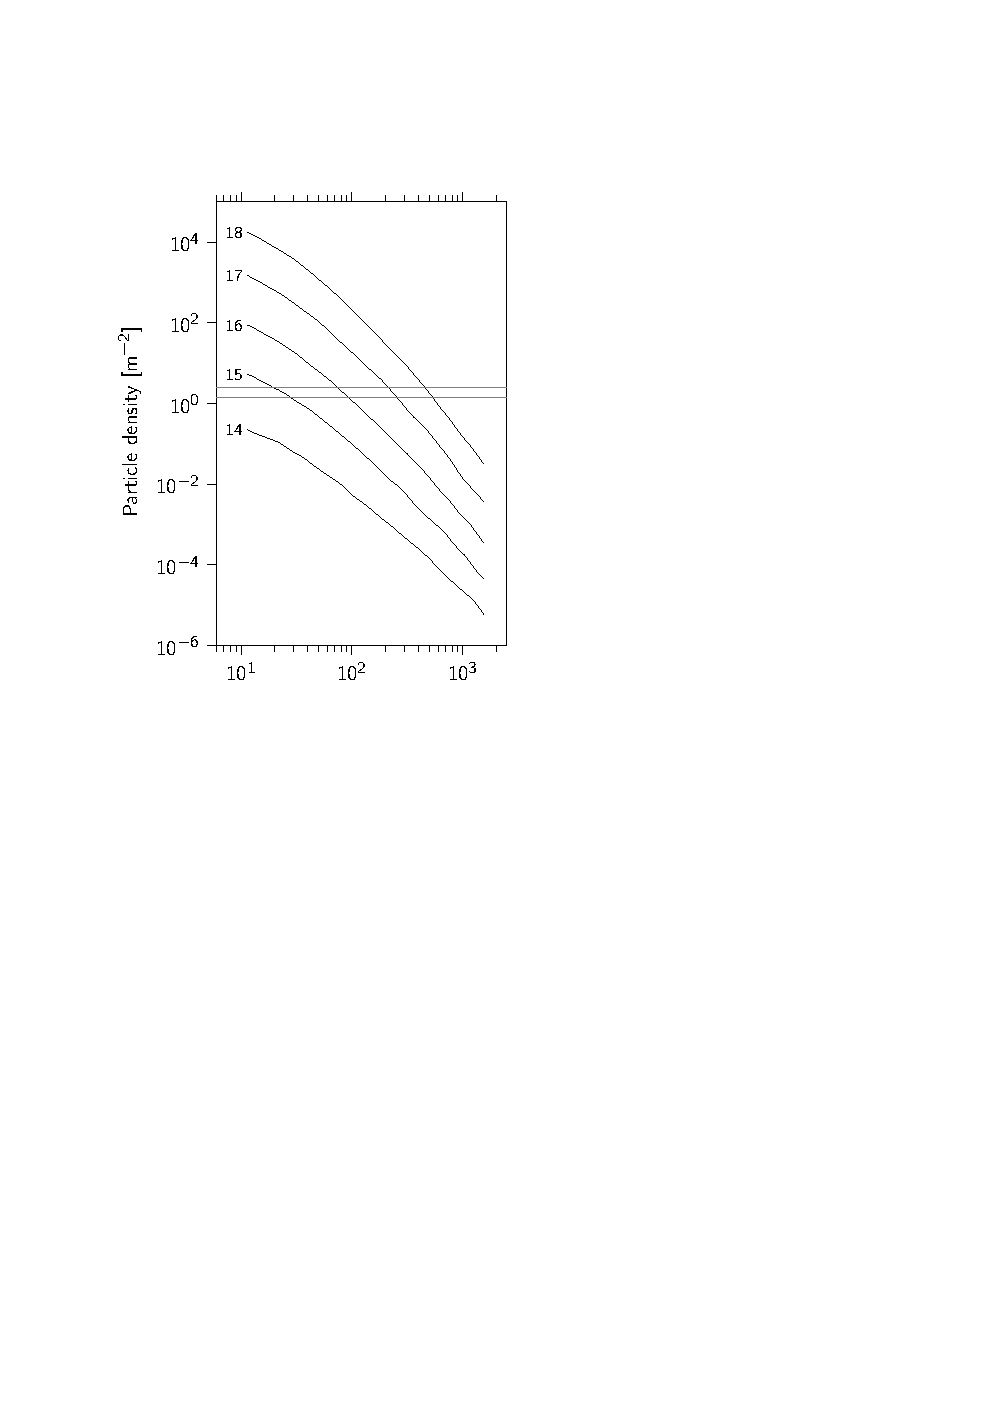
\includegraphics[width=0.6\textwidth]
                    {plots/experiment/ldf_energies}
    \caption{Trigger efficiency E = \SIrange{e14}{e20}{\eV} showers, add horizontal lines for 2 in 2-detector, any 2 in 4-detector, and any 3 in 4-detector (\SI{50}{\percent} efficient.}
    \label{fig:ldf_energies2}
\end{figure}

% Explain simple direction reconstruction with 3 detection points (flat/curved shower).
When there are three detection points which are not on a line the shower axis can be constrained. In this case the detectors are assumed to be at the same height and the front is considered flat, an approximation which can be valid at the short distances between detectors as they occur in a station.
[derivation of formula for shower direction, cartesian, 2D, flat]

\subsection{Station layout}
\label{ssec:station_layout}

% Standard layouts created to encourage uniformity, these are also chosen for good shower acceptance, reconstruction accuracy of station events, and practicality for the locations.
The layouts of a typical 4-detector station is shown in \cref{fig:4_detector_layouts}. The detectors are separated by \SI{10}{\meter} to exclude the smallest showers and provide accurate direction reconstruction resolution. Given the location of the station is on the roofs of buildings the size of typical roofs also limits the possible size of the stations. The distance between detectors also affects the resolution for reconstructing the direction of air showers. The possible directions for three detectors in an equilateral triangle with \SI{10}{\meter} sides and a timing resolution of \SI{2.5}{\ns} is shown in \cref{fig:discrete_directions}. Using the inner detector with two outer detectors reduces the direction resolution, having only 1/3rd the possible directions. In some cases (space allowing) the decision has been made to move the inner detector outside the triangle to form a second equilateral triangle sharing one of the sides. In this case all combinations of three detectors result in the same possible direction reconstructions.

\begin{figure}
    \centering
    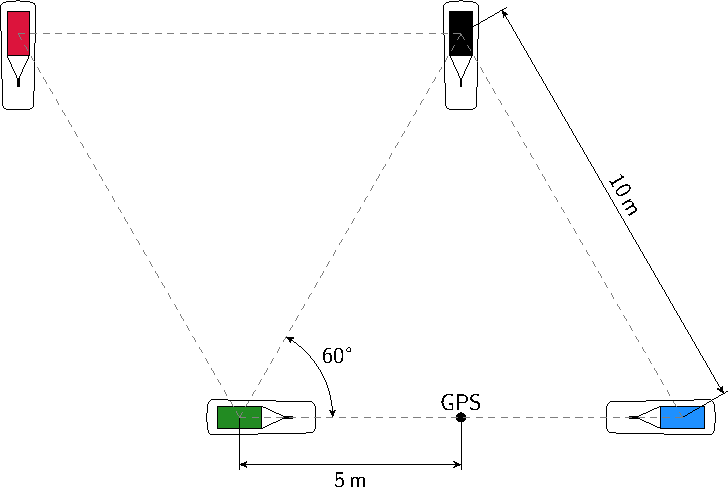
\includegraphics[width=0.4\textwidth]
                    {plots/experiment/4_detector_diamond}
    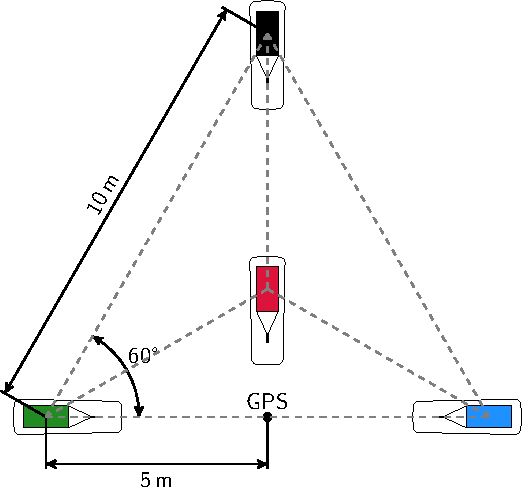
\includegraphics[width=0.4\textwidth]
                    {plots/experiment/4_detector_star}
    \caption{4-detector station layouts. 4-detector stations are typically placed in the diamond or star formation. Both contain multiple triangles between sets of 3 detectors.}
    \label{fig:4_detector_layouts}
\end{figure}

\begin{figure}
    \centering
    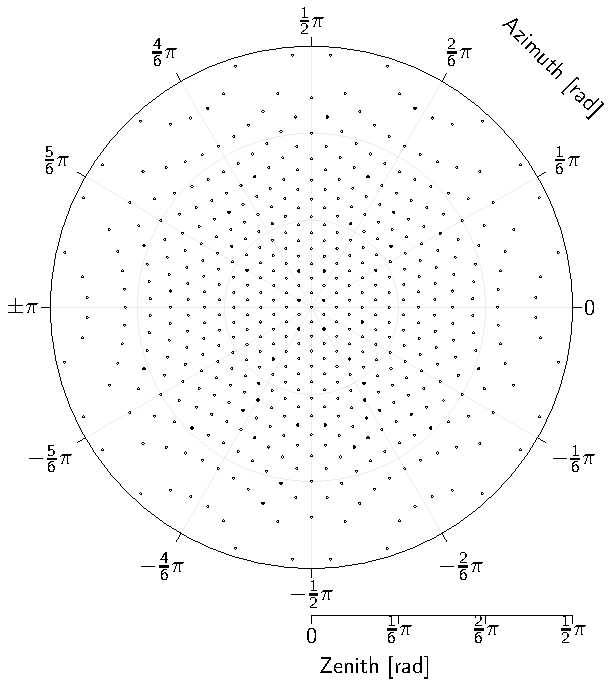
\includegraphics[width=0.6\textwidth]
                    {plots/experiment/discrete_directions}
    \caption{Both 4-detector layouts result in the following distribution of possible shower directions given \SI{2.5}{\ns} arrival time sampling in the detectors. For the diamond layout more points can be made by more combinations, i.e. more possible solutions. Approximately \SI{5}{\degree} between adjacent points near Zenith.}
    \label{fig:discrete_directions}
\end{figure}

The layout of each station is not always precisely according to the suggested layout. Not all roofs provide the required space. It is not a problem if the layout deviates from the suggested ones, as long as the actual positions are known. In order to get the absolute position of the detectors their positions are measured relative to the \gps, whose position is know. From the \gps the distance to and the angle between (True?) North and the detector (center of the scintillator) is measured. Additionally the rotation of the detector itself around its center can be recorded, though this is less important. The coordinate system is also described in \cref{ch:coordinates}. If the location of detectors relative to the \gps is changed the new layout can be recorded with the timestamp of when it changed. The data analysis takes these changes into account to use the correct layout when reconstructing events. For students a document has been created which outlines the steps for measuring their detector positions and how they can submit them to the Public Database. Information about the position of detectors in 2-detector stations is also important. Though full direction reconstruction is not possible with only two detectors it can define a plane where the shower should come from (reference Niek).

% Shower core/energy determination impractical with single station.
Determination of the shower core is impractical with a single station. The error on the determination of the particle density is to high and the number of detection points to low.

\subsection{Weather station}

% Optional weather station to provide local weather data.
Optionally a \hisparc station can be extended with a weather station to provide local weather measurements. These measurements can help in understanding how shower development is affected by atmospheric conditions. For instance an high air pressure increases the number of collisions in air showers, thereby reducing the number of particles that reach sea level. This lowers the trigger rate for a station. Additionally some of the detector components have efficiencies dependent on their temperature. By measuring the temperature detections may be corrected for the changed efficiency. \hisparc uses a VantagePro weather station which includes the following sensors; temperature, air pressure, humidity, solar radiation, wind direction, wind speed, rain, and . These sensors are readout every \SI{5}{\second}. Currently there are .. \hisparc stations that also have a weather station. These locations are shown on the map in [fig ref].

% May not be required at each station, can use freely available KNMI data. However, in some cases closest KNMI station is far away.
Note that it is not required for all stations to have a weather station. The Royal Dutch Meteorological Institute (KNMI) also provides a public weather data service in the Netherlands. KNMI has 36 stations spread in a regular grid around the Netherlands. Not all \hisparc stations are close to a KNMI station, for some weather quantities this is no problem because they are similar over long distances, or can be interpolated. Besides temperature the local solar radiation strongly influences the temperature of the detector in a skibox.

\begin{figure}
    \centering
    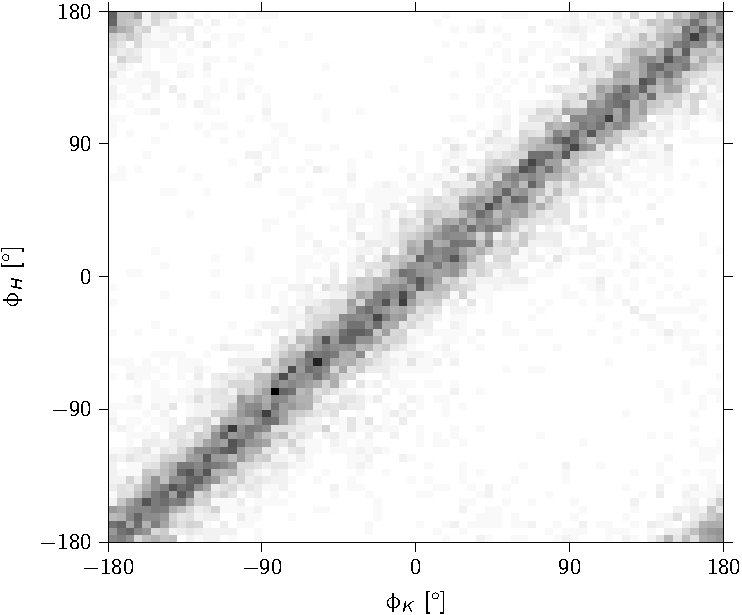
\includegraphics[width=0.6\textwidth]
                    {plots/experiment/azimuth_kascade_minn1}
    \caption{Test station at KASCADE was used to verify the performance of a single station. The direction agreement between simultaneously detected events is shown.}
    \label{fig:azimuth_kascade_minn1}
\end{figure}


\begin{figure}
    \centering
    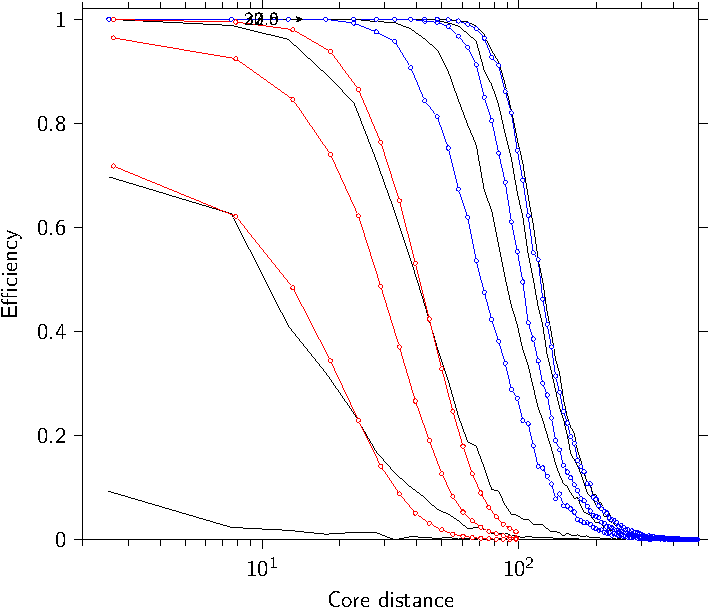
\includegraphics[width=0.6\textwidth]
                    {plots/experiment/efficiency_two_16}
    \caption{Detection (trigger) efficiency as a function of core distance for showers of different primary energy (and zenith).}
    \label{fig:efficiency_two_16}
\end{figure}


\begin{figure}
    \centering
    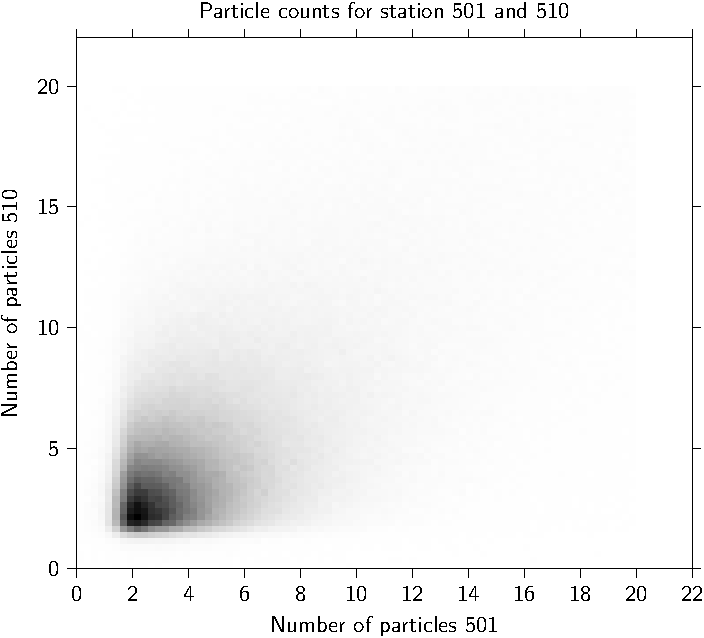
\includegraphics[width=0.6\textwidth]
                    {plots/experiment/n_501_510_sum}
    \caption{(place holder figure showing different data) Test station at KASCADE used to verify the particle density measurement of a single detector and full station, compared to the KASCADE predicted particle density.}
    \label{fig:n_501_510_sum}
\end{figure}


\section{Network}

% How the network started, when stations were built.
In 2004 \hisparc started data collection. Initially with several stations in Amsterdam, later expanding to other regions. Over the last \SI{12}{\year} the number of stations with data has grown at a rate of approximately one per month. Unfortunately not all stations continue to operate properly. \cref{fig:active_stations} shows the number of stations that have had at least a days worth of events (green), additionally it shows the number of active stations per day (black). Though the number of active station has also increased it lags behind the total number of stations. This is partially explained by stations being moved to a new location under a new name. In which case both stations count toward the total number of stations, but only one active station. In some cases the contact at a station retired and no followup was arranged, leaving the station without proper maintenance. In other cases problems have been known to be caused by Windows Updates, internet proxies, bad configuration, power supply failures, light leaks in the detectors, or many other issues have caused stations to be down. In many cases remote control of the station can be used to make station operational again.

\begin{figure}
    \centering
    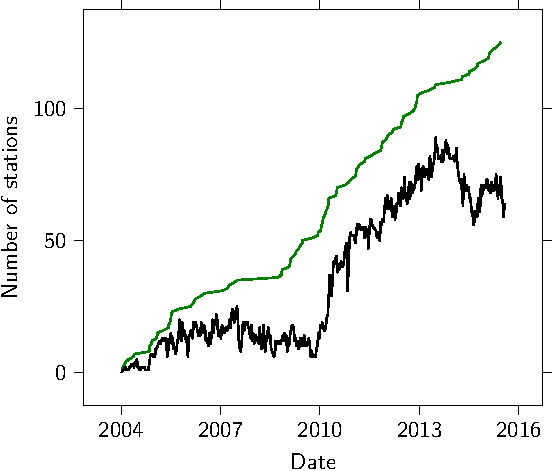
\includegraphics[width=0.6\textwidth]
                    {plots/experiment/active_stations}
    \caption{Cumulative number of stations with at least an hour of good data and the number of active stations per day.}
    \label{fig:active_stations}
\end{figure}

% Each station submits data/triggered events to central datastore
When a station records data is uploads it to the central datastore at \nikhef. Here further offline analysis is performed and the data is made available for download. The automatic data analysis that is performed is described in [a later chapter]. The data is sent from the station as a HTTP POST request to the datastore server. This server checks the station number and password for verification and if all data is correctly uploaded using a checksum. If this succeeds the data is stored in the raw datastore. The datastore stores the detected events, comparator data, configuration settings, error messages, single rates, and \gps signal information. Additionally a station may upload weather data, for which the data, configuration and errors are stored. In \cref{fig:luminosity_network} the cumulative number of detected events (green) and verified good events (black) are shown.

\begin{figure}
    \centering
    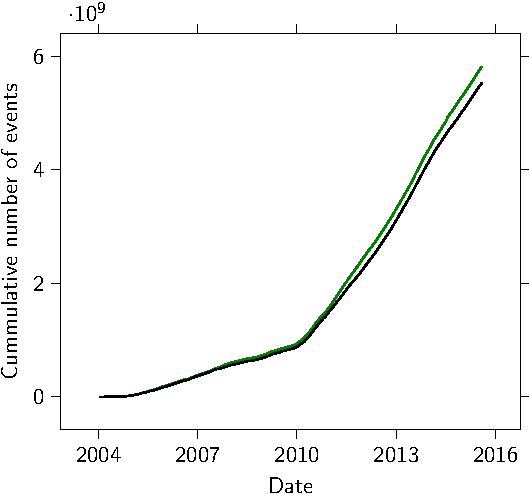
\includegraphics[width=0.6\textwidth]
                    {plots/experiment/luminosity_network}
    \caption{Cumulative number of events by all stations, the lower line contains only events when the stations were working properly.}
    \label{fig:luminosity_network}
\end{figure}

% Use offline analysis to find station events detecting the same shower.
  % - This requires good absolute timing at the stations.
  % - Use GPS at stations for both positioning of the stations (\SI{~1}{\meter}) and absolute timing (\SI{~5}{\ns}).
An `offline trigger' is used to determine when stations were probably detecting the same shower. This is similar to the station trigger. In this case the data is searched for (at least two) stations that simultaneously (i.e. within a certain time window) detected events. These events that are likely due to the same shower are called coincidences. Coincidences between stations are expect to be caused by either the detection of the same shower, the detection of separate but correlated showers (due to the GZ-effect), or the detection of two unrelated showers. The absolute timing of events detected by stations is important when looking for coincidences. It also influences the resolution with which coincidences can be reconstructed, because the arrival times in the detectors of the stations is to be compared.

\subsection{Station locations}

% Current station locations, explain why the stations are in those locations. Due to those being the locations of high schools..
In [fig ref to map of station locations] the locations of all \hisparc stations is shown. In most regions there are multiple stations close (? km?) to each other. The locations are in most cases limited to the locations of high schools and universities. Local universities provide support for the high schools, they guide students in building the detectors and provide support when needed. There are currently about \num{650} high schools in the Netherlands, some of which have multiple locations, resulting in a total of about \num{1500} school locations. Currently there are \num{80} high schools participating in \hisparc.

\subsubsection{International}

Locations of \hisparc stations are not limited to the Netherlands. Two other countries successfully operate multiple detection stations. All station locations are shown in \cref{fig:network}.

Since 2007 there has been a \hisparc station in Denmark. There are currently 3 operational stations at the Aarhus University. These stations are managed by Uffe Amelung Fredens. Fredens also wrote student materials for Danish high school students.

In the United Kingdom a new cluster in Bristol was started in March 2012. This was initiated by Dr. Jaap Velthuis. Dr. Velthuis is the cluster coordinator for the Bristol cluster. Since then any schools around Bristol have created detectors and joined the network. Even more schools have plans to join. In 2014? a second cluster has started in the United Kingdom around Birmingham. The Birmingham cluster is coordinated by Cristina Lazzeroni.

In Germany a station (70001) was temporarily placed inside the \kascade experiment in Karlsruhe. This was done to calibrate and test the direction reconstruction accuracy of a single \hisparc station. Although the \kascade-GRANDE experiment officially shut down on March 30, 2009, it was kept active until November, 26th 2011 as a test facility for some test setups, including our detection station. \kascade triggered the \hisparc station when it detected a shower. More than \num{9e7} triggers occurred [in publicdb, more on external hdd? and in `/databases/kascade'?] in this period. The detectors used for the \kascade station have since been repurposed and now form station 508 on the Science Park.

\begin{figure}
    \centering
    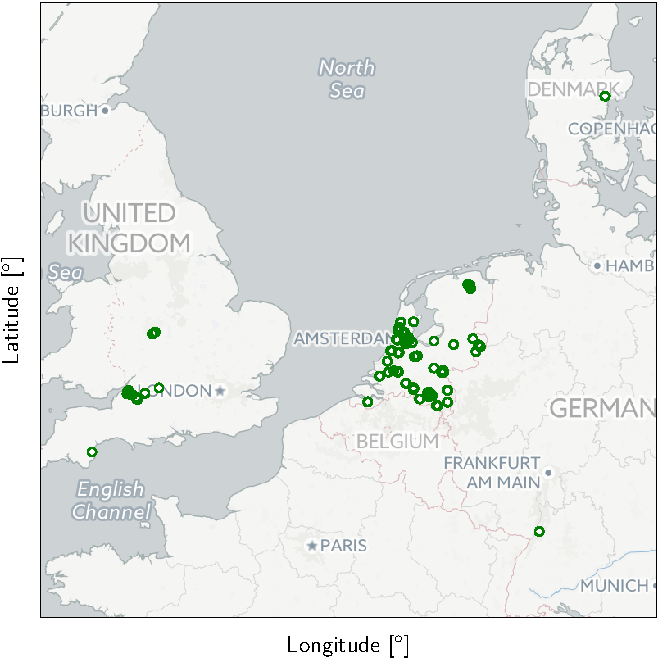
\includegraphics[width=0.6\textwidth]
                    {plots/experiment/network}
    \caption{Locations of HiSPARC stations in Netherlands, United Kingdom, and Denmark. Stations which also include a weather station are indicated with red circles.}
    \label{fig:network}
\end{figure}

Interesting for shower reconstruction, coincidence rate, and possibilities for detection the GZ-effect are the distances between pairs of stations. In \cref{fig:network_station_distances} the distribution of distances between all possible pairs of stations are shown. The points beyond \SI{250}{\kilo\meter} are due to combinations between stations in the Netherlands and the international stations. And the pair separated by only \SI{2}{\meter} is the combination of station 501 and 510. These were specifically placed to compare the results from two stations which are virtually at the same location. The results from comparing these stations is shown in [ref to later chapter about station performance or reconstructions].

\begin{figure}
    \centering
    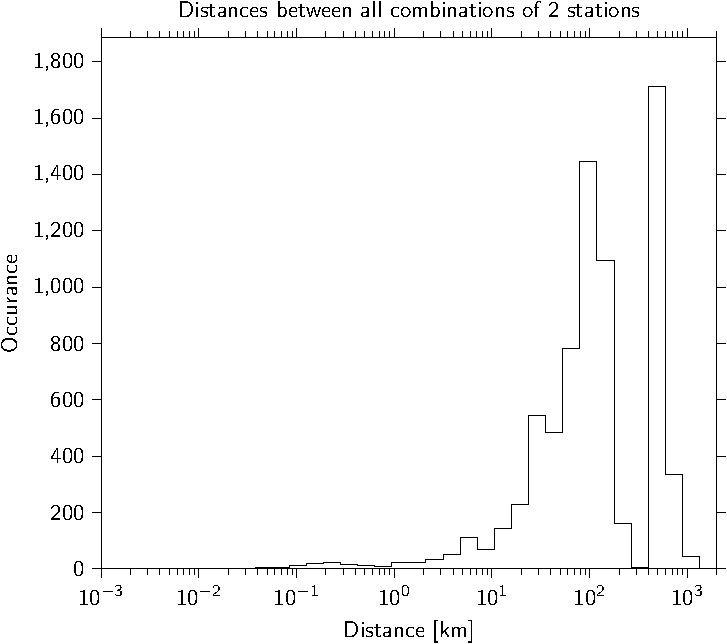
\includegraphics[width=0.6\textwidth]
                    {plots/experiment/network_station_distances}
    \caption{Distribution of distances between all possible pairs of stations in the entire HiSPARC network.}
    \label{fig:network_station_distances}
\end{figure}

\subsection{Coincidence rate}

% Stations closer than \SI{2e3}{\meter} are likely to at some point detect the same shower.
For stations up to \SI{2e3}{\meter} distance from each other they are likely to detect the same shower at some point in time. However, the rate is so low that is approaches the rate coincidences due to random background particles. Large showers which can be detected up to \SI{e3}{\meter} from the shower core have energies of at least \SI{e18}{\eV}. [estimate the coincidence rate for showers of certain energy.]

In \cref{fig:distance_v_coincidence_rate} the coincidence rate is determined for all pairs of stations. Counting only the time that both stations were working properly. The determined coincidence rate is then plotted against the distance between the stations. The different coincidence rates due to detection efficiencies caused by the different number of detectors in stations is expected. The different combinations of two 2-detector, two 4-detector, and a 2- and 4-detector stations are indicated by different symbols. The background rate is estimated by \cref{eq:background_rate} and indicated by the horizontal dashed lines.

\begin{figure}
    \centering
    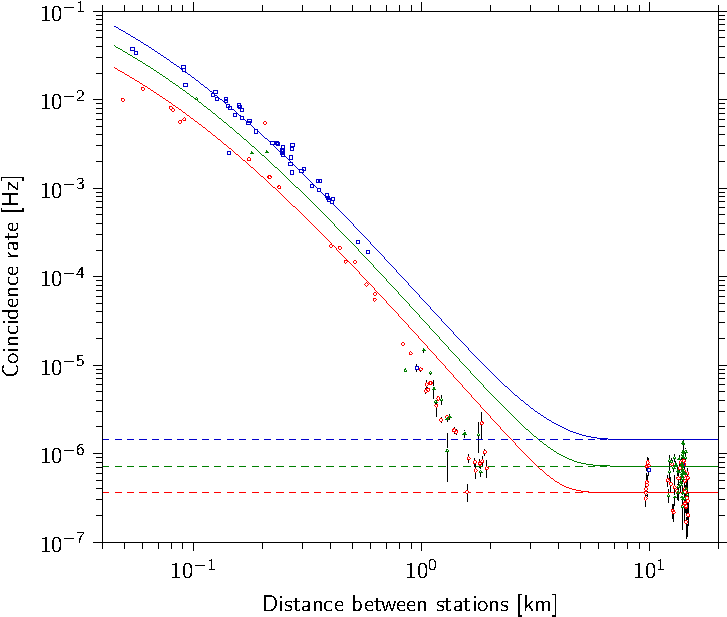
\includegraphics[width=0.6\textwidth]
                    {plots/experiment/distance_v_coincidence_rate}
    \caption{Coincidence rate between stations as a function of distance. At increasing distances the contributions from increasingly larger/energetic showers dominate. The background rate is also shown (dashed). Real events may still be distinguished from background. The square indicates two 4-detector stations, triangle for a 4- and 2-detector station, and the circle two 2-detector stations.}
    \label{fig:distance_v_coincidence_rate}
\end{figure}

\subsection{Shower reconstruction with multiple stations}

% Similar direction reconstruction algorithm as used for single station.
With the combined measurement data from multiple stations a more accurate reconstruction is possible. The distances between the detection points are larger while the timing accuracy remain excellent. The reconstruction algorithm needs to take into account the different relative altitudes of the detectors, these are no longer all at the same altitudes.

% At large core distances the curvature of the shower front should be taken into account.
Moreover, the curvature and rise time of the shower front plays a bigger role and needs to be accounted for in the reconstruction.

- For a large event should arrival times in each detector be used or station average density and average/first arrival time?

\begin{figure}
    \centering
    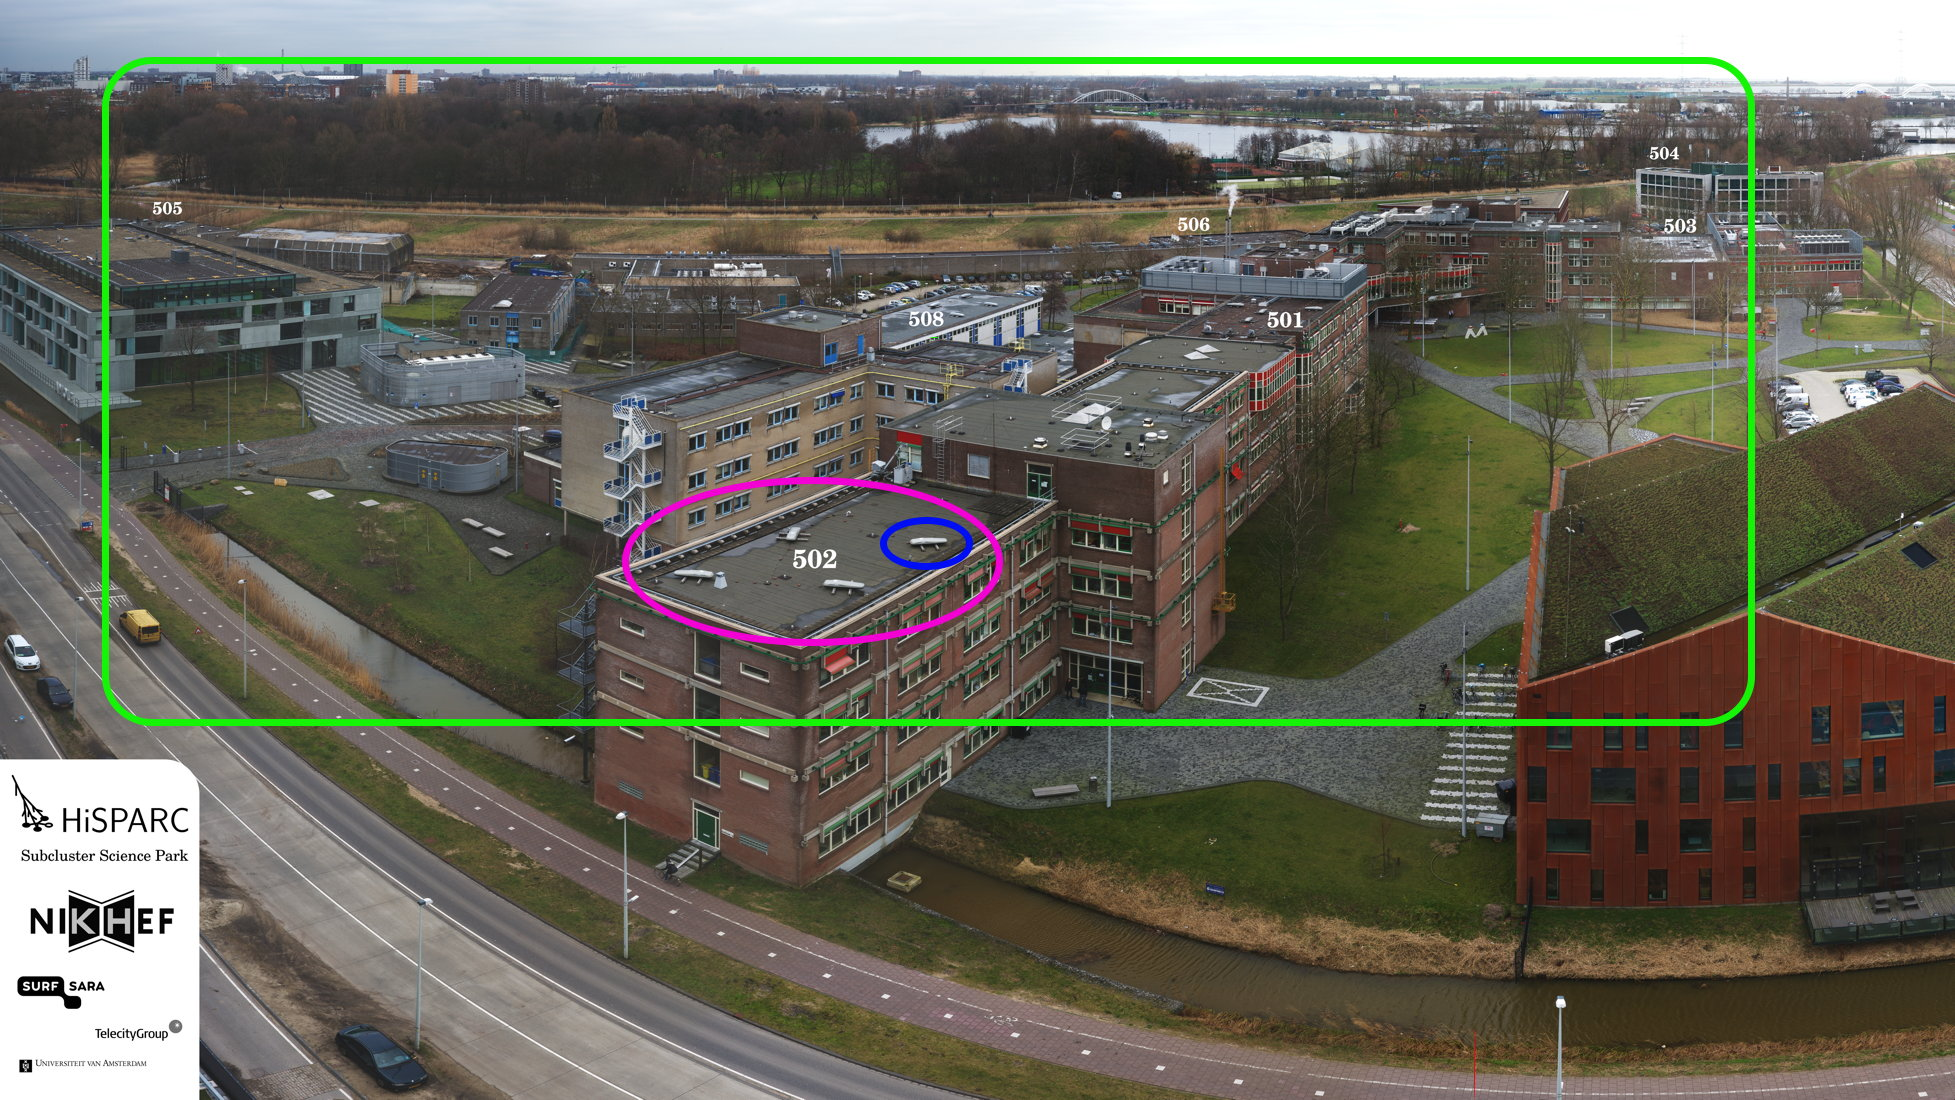
\includegraphics[width=0.6\textwidth]
                    {plots/experiment/ADL_151373_151429_layers.jpg}
    \caption{Show what a collection of stations look like. Highlight a single detector, a station, and a collection of stations.}
    \label{fig:ADL_151373_151429_layers}
\end{figure}




\begin{figure}
    \centering
    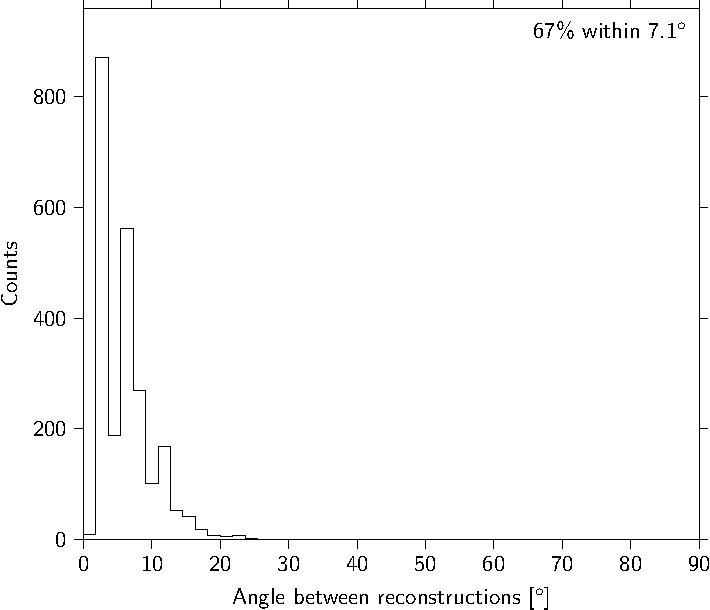
\includegraphics[width=0.6\textwidth]
                    {plots/experiment/angle_between_501_minn16_510}
    \caption{(placeholder plot, not data mentioned in caption) Distance between reconstructions when using average/first arrival time, versus simulation input. Using separate detectors should hold more information, but the reconstruction algorithm should be aware (using curved or flat reconstruction?)}
    \label{fig:angle_between_501_minn16_510}
\end{figure}
